% Dataset pipeline (Ch. 3). Compile with pdfLaTeX/Tectonic; copy data-pipeline.pdf to figures/.
\documentclass[12pt,border=2pt]{standalone}
\usepackage[T1]{fontenc}\usepackage{newtxtext}
\usepackage{tikz}\usetikzlibrary{positioning,arrows.meta,calc}
\begin{document}
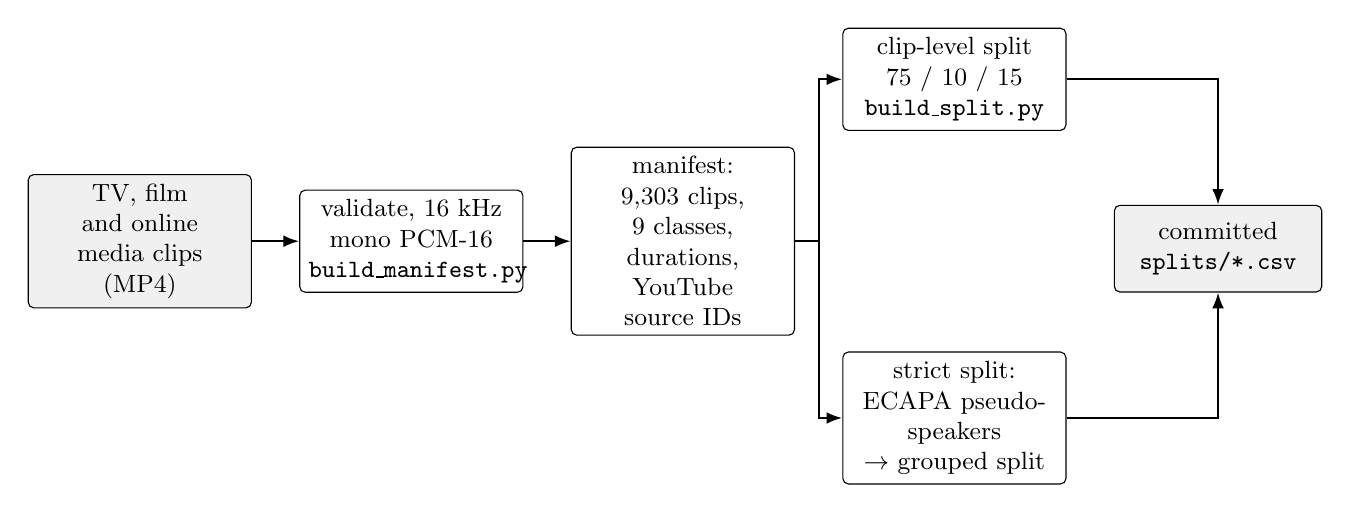
\begin{tikzpicture}[node distance=4mm and 6mm,
  box/.style={draw, rounded corners=2pt, align=center, font=\small, minimum height=11mm, text width=26mm, fill=white},
  data/.style={box, fill=black!6}, arr/.style={-{Latex[length=2mm]}, thick}]
  \node[data] (raw) {TV, film and online\\media clips (MP4)};
  \node[box, right=of raw] (std) {validate, 16 kHz\\mono PCM-16\\\texttt{build\_manifest.py}};
  \node[box, right=of std] (man) {manifest: 9,303 clips,\\9 classes, durations,\\YouTube source IDs};
  \node[box, above right=2mm and 6mm of man] (clip) {clip-level split\\75 / 10 / 15\\\texttt{build\_split.py}};
  \node[box, below right=2mm and 6mm of man] (strict) {strict split:\\ECAPA pseudo-speakers\\$\rightarrow$ grouped split};
  \node[data, right=6mm of $(clip.east)!0.5!(strict.east)$, text width=24mm] (out) {committed\\\texttt{splits/*.csv}};
  \draw[arr] (raw) -- (std); \draw[arr] (std) -- (man);
  \draw[arr] (man.east) -| ($(man.east)+(3mm,0)$) |- (clip.west);
  \draw[arr] (man.east) -| ($(man.east)+(3mm,0)$) |- (strict.west);
  \draw[arr] (clip.east) -| (out.north); \draw[arr] (strict.east) -| (out.south);
\end{tikzpicture}
\end{document}
